Пока что, в контексте выбранной модели, хуже всего можем оценить $l$, поэтому будем сравнивать теоритескую и экспериментальную оценку $\kappa$ по значению $l$  при котором они бы сходились:
\begin{equation*}
    l = \underbrace{\frac{\log 1/\beta_0}{F[0, \nu_0]}}_{\kappa} \frac{\sqrt{\pi}}{n \sigma_0} \underbrace{\sqrt{\frac{2 \sub{k}{Б} T}{m}}}_{v_0}.
\end{equation*}
Считая $\sigma_0 = \sigma_0^{\text{теор}}$, построим зависимость $l[\beta]$, рис. \ref{fig:lx}.

\begin{figure}[h]
    \centering
    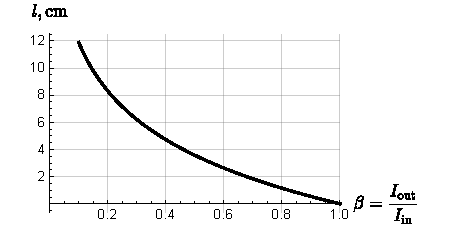
\includegraphics[width=0.5\textwidth]{"D:\\Kami\\git_folder\\notes_5sem\\rqc\\saturation_spectr_simulation\\lx.pdf"}
    \caption{Оценка длины взаимодействия лазера с литием при температуре в $300\ {}^{\circ}$С}
    \label{fig:lx}
\end{figure}
